\documentclass[12pt]{article}
\usepackage{latexblog}

% ============================================================
% Blog Metadata
% ============================================================
\blogtitle{阅读笔记：HashMap}
\blogdate{2020-03-18}
\blogtags{刨根问底, 探索分析, JDK1.8}
\bloglang{zh}
\blogsummary{}

\begin{document}
\makeblogtitle

HashMap可以算是最常用的数据结构了，而它的实现没想到还挺有学问在里面。

\section{基本实现}\label{ux57faux672cux5b9eux73b0}

\subsection{哈希映射}\label{ux54c8ux5e0cux6620ux5c04}

在HashMap中使用数组来存储元素，根据元素的hash值一一映射到一个节点上。其中使用的哈希方法为：

\begin{Shaded}
\begin{Highlighting}[]
\DataTypeTok{static} \DataTypeTok{final} \DataTypeTok{int} \FunctionTok{hash}\OperatorTok{(}\BuiltInTok{Object}\NormalTok{ key}\OperatorTok{)} \OperatorTok{\{}
    \DataTypeTok{int}\NormalTok{ h}\OperatorTok{;}
    \CommentTok{// 将哈希值无符号右移16位是因为取index使用了length作为掩码，这样当哈希值在掩码外的部分相同的时候就会发生冲突}
    \CommentTok{// 这样将高位混杂到低位上，可以尽可能将这种影响消除}
    \ControlFlowTok{return} \OperatorTok{(}\NormalTok{key }\OperatorTok{==} \KeywordTok{null}\OperatorTok{)} \OperatorTok{?} \DecValTok{0} \OperatorTok{:} \OperatorTok{(}\NormalTok{h }\OperatorTok{=}\NormalTok{ key}\OperatorTok{.}\FunctionTok{hashCode}\OperatorTok{())} \OperatorTok{\^{}} \OperatorTok{(}\NormalTok{h }\OperatorTok{\textgreater{}\textgreater{}\textgreater{}} \DecValTok{16}\OperatorTok{);}
\OperatorTok{\}}
\end{Highlighting}
\end{Shaded}

举例来说对于容量为4的HashMap，插入''a''、``b''、``c''、``d''后在数组中的分布就是：

\begin{Shaded}
\begin{Highlighting}[]
\StringTok{"a"}\OperatorTok{.}\NormalTok{hashCode}\OperatorTok{()} \OperatorTok{=} \DecValTok{97} \OperatorTok{=} \DecValTok{00000000000000000000000001100001}
\NormalTok{hash}\OperatorTok{(}\StringTok{"a"}\OperatorTok{)} \OperatorTok{=} \DecValTok{00000000000000000000000001100001} \OperatorTok{\^{}} \DecValTok{00000000000000000000000000000000}
          \OperatorTok{=} \DecValTok{00000000000000000000000001100001}
\VariableTok{index} \OperatorTok{=}\NormalTok{ hash}\OperatorTok{(}\StringTok{"a"}\OperatorTok{)} \OperatorTok{\&} \OperatorTok{(}\DecValTok{4} \OperatorTok{{-}} \DecValTok{1}\OperatorTok{)}
      \OperatorTok{=} \DecValTok{00000000000000000000000001100001} \OperatorTok{\&} \DecValTok{00000000000000000000000000000011}
      \OperatorTok{=} \DecValTok{00000000000000000000000000000001}
\end{Highlighting}
\end{Shaded}

如此则数组中对应的序号为1，2，3，0。

\begin{figure}
\centering
\pandocbounded{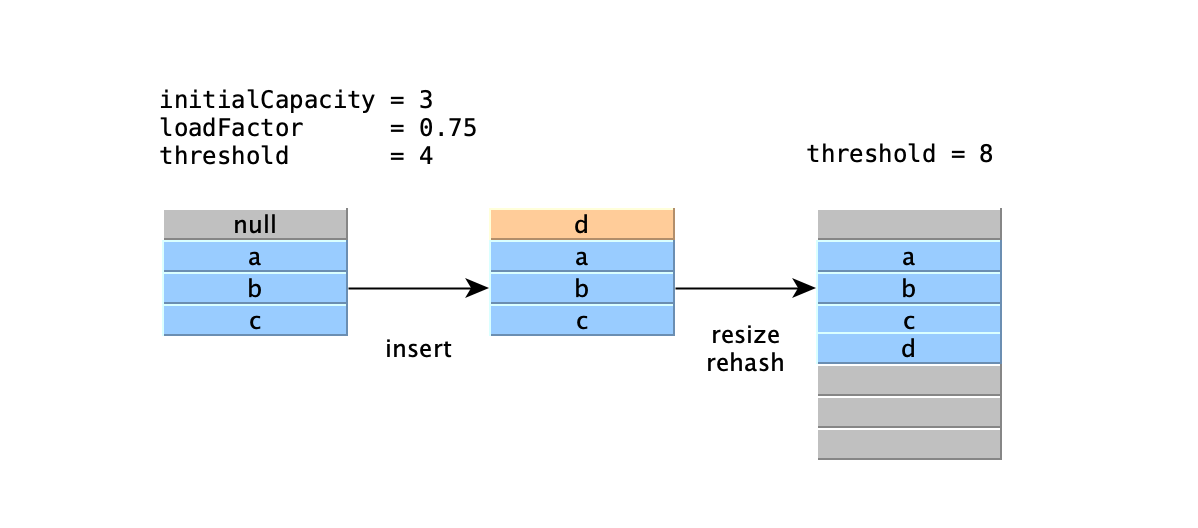
\includegraphics[keepaspectratio,alt={HashMap resize}]{images/HashMap-resize.png}}
\caption{HashMap resize}
\end{figure}

\subsection{Load Factor(负载因子)和Threshod（阈值）}\label{load-factorux8d1fux8f7dux56e0ux5b50ux548cthreshodux9608ux503c}

因为HashMap的底层实际上是使用数组进行存储，那么始终存在着一个动态内存分配的问题：数组的大小是固定的，但是HashMap实际存储多少数据是未知的（可以一直向HashMap中进行插入），那么当数组塞满了（实际上还有一个问题是发生哈希冲突）之后如何处理？

解决这个问题最简单的做法就是，一旦数组满了之后，就对数组进行扩容。扩容也很简单，重新申请一个大一点的数组，再把原来数组里面的数据复制过去即可。这里涉及到另外一个问题就是，扩容的时候选择一个怎么样的容量进行扩容呢？这个操作是有代价的，如果频繁的扩容就涉及到频繁的数组复制操作，性能上会受到影响；如果一次扩容选择一个很大的空间，但实际之后这些空间又没有使用到，那么久造成了资源浪费。怎么解决这一个问题呢？

在HashMap的构造中有两个关键的参数：

\begin{itemize}
\tightlist
\item
  \texttt{initialCapacity}:初始化容量，即可以装多少条数据
\item
  \texttt{loadFactor}：负载因子，用来描述HashMap中可以变得多``满''（到达什么程度开始扩容）
\end{itemize}

实际上，HashMap并不会根据你提供的\texttt{initial\ capacity}来初始化一个数组，而是找到一个值 \(t\) 并满足 \(t >= i \&\& t==2^{n}\)（比如3对应得到4， 15对应得到16），并在第一次插入的时候进行初始化。

为什么数组在初始化的时候一定是2的倍数？这是因为方便扩容的时候直接将数组大小变成原来的二倍，同时也简化了一些其他的操作，比如如何定位到一个值所在的索引:

\begin{Shaded}
\begin{Highlighting}[]
\DataTypeTok{int}\NormalTok{ index }\OperatorTok{=} \OperatorTok{(}\NormalTok{length }\OperatorTok{{-}} \DecValTok{1}\OperatorTok{)} \OperatorTok{\&}\NormalTok{ hash}

\CommentTok{/*}
\CommentTok{final Node\textless{}K,V\textgreater{} getNode(int hash, Object key) \{}
\CommentTok{    Node\textless{}K,V\textgreater{}[] tab; Node\textless{}K,V\textgreater{} first, e; int n; K k;}
\CommentTok{    if ((tab = table) != null \&\& (n = tab.length) \textgreater{} 0 \&\&}
\CommentTok{        (first = tab[(n {-} 1) \& hash]) != null) \{}
\CommentTok{    ...}
\CommentTok{*/}
\end{Highlighting}
\end{Shaded}

正常的做法是，\texttt{abs(hash)\ \%\ SIZE}像这样取余操作。但是如果除数是2的n次幂，则可以简化为位运算操作。

而至于为什么默认的负载因子是0.75，有人根据二项式分布算出最佳的load factor是 \(log(2)=0.693\) ，然后拍脑袋给出的0.75（乘以容量还可以得个整数\ldots)。

\section{树化（红黑树）}\label{ux6811ux5316ux7ea2ux9ed1ux6811}

\subsection{TREEIFY\_THRESHOLD（树化阈值）}\label{treeify_thresholdux6811ux5316ux9608ux503c}

所以使用0.75作为负载因子，那么出现的情况是如果当前容量达到这个值的时候就会resize到原来的两倍。对于一个容量为4的Map来说，理想情况下元素均匀分布，是这样：

\begin{verbatim}
最好情况                                 极端情况
bucket | elements                      bucket | elements     
-------+---------                      -------+---------    
     0 | Z                                  0 |   
     1 | X                                  1 | Z -> X -> Y 
     2 |                                    2 |  
     3 | Y                                  3 | 
\end{verbatim}

理想状况下（假设基于随机hash算法节点在桶中均匀分布，且节点的个数占桶的50\%，那么单个节点出现在桶中的概率为0.5），节点在hash桶中的出现的频率遵循\href{https://zh.wikipedia.org/wiki/\%E6\%B3\%8A\%E6\%9D\%BE\%E5\%88\%86\%E4\%BD\%88}{泊松分布}（ \(λ = 0.5\) )

\[
P(X=k)=\frac{e^{-\lambda}\lambda^k}{k!}=\frac{e^{-0.5}0.5^k}{k!}
\]

意味着在load factor=0.75的情况下，hash桶中出现 \(k\) 个节点（冲突）的概率大致为：

\begin{verbatim}
* 0:    0.60653066
* 1:    0.30326533
* 2:    0.07581633
* 3:    0.01263606
* 4:    0.00157952
* 5:    0.00015795
* 6:    0.00001316
* 7:    0.00000094
* 8:    0.00000006
* more: less than 1 in ten million
\end{verbatim}

可见哈希冲突导致一个桶中出现8个节点情况已经几乎小之又小的事情了，这是\texttt{TREEIFY\_THRESHOLD\ =\ 8}的原因，当大于8的时候转换为红黑树。

\subsection{Treeify（树化）}\label{treeifyux6811ux5316}

通常情况下，当哈希冲突产生的时候，会被当成链表存储。这个改变是通过\href{http://openjdk.java.net/jeps/180}{JEP 180: Handle Frequent HashMap Collisions with Balanced Trees}引入的。在下面的情况下，会转换为红黑树：

\begin{itemize}
\tightlist
\item
  链表中的节点数达到TREEIFY\_THRESHOLD（8）
\item
  容量至少达到MIN\_TREEIFY\_CAPACITY（64），否则只是单纯扩容到到原来的两倍
\end{itemize}

现实中哈希冲突的场景并不多，不过如果非要测试这种场景也很容易。比如\texttt{Aa}和字符串\texttt{BB}就拥有相同的哈希值，把他们随机组合到一起，还是一样。于是我们构建了很多个哈希值相同的key值，来演示哈希冲突的场景：

\begin{figure}
\centering
\pandocbounded{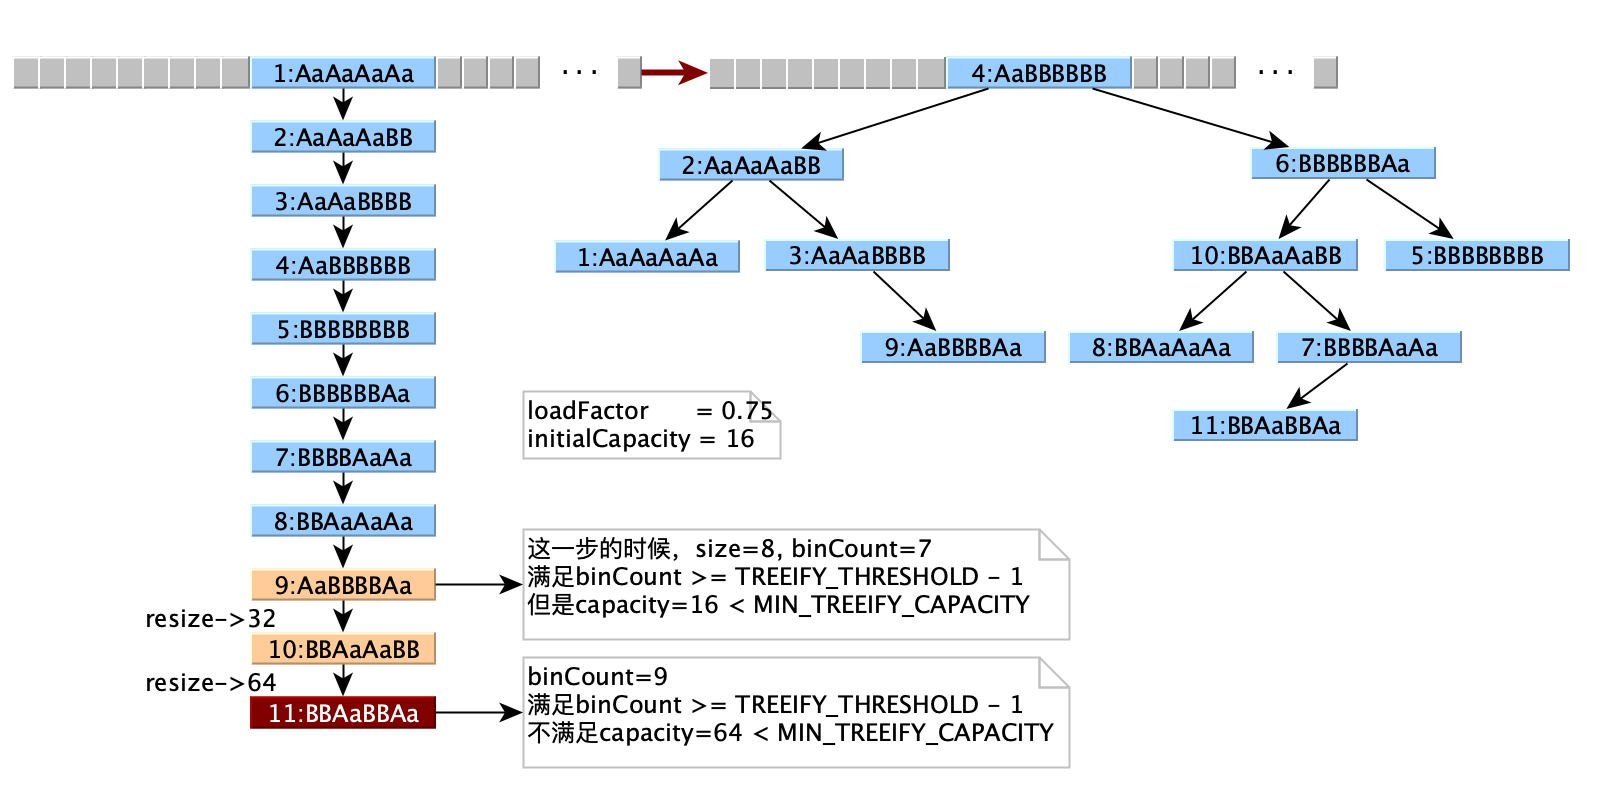
\includegraphics[keepaspectratio,alt={Treeify}]{images/HashMap-treeify.png}}
\caption{Treeify}
\end{figure}

\subsection{尾插入}\label{ux5c3eux63d2ux5165}

从上面的图可以注意到：哈希冲突的节点在链表中是插入到链表尾部的

在Java8之前是插入到前面的，但是Java8改成插入到尾部了，这样做的原因（据说）是因为扩容时会改变链表的顺序，在多线程条件下会导致形成闭环（从而可能引起死循环）。

\section{fail-fast机制}\label{fail-fastux673aux5236}

在HashMap中存在一个变量记录修改的次数\texttt{modCount},当这个次数和期待的不一致的时候就会抛出\texttt{ConcurrentModificationException}。这种机制被称之为''Fail-Fast''，意味着出现错误的时候尽早结束。通常在\texttt{java.util}下面的迭代器都是这类的，如果在迭代的中途数据被其他线程修改了，那么就会（尽可能的，当然并不能保证）触发这个检测。

而\texttt{java.util.concurrent}包下的迭代器是''Fail-Safe''的，例如ConcurrentHashMap、CopyOnWriteArrayList等。

\section{性能分析}\label{ux6027ux80fdux5206ux6790}

HashMap对于\texttt{get}和\texttt{put}操作的复杂度是常数级 \(\displaystyle{O(1)}\) ，在最坏的情况下，因为使用了红黑树进行查找，复杂度为 \(\displaystyle{O(log(n))}\) 。

\begin{itemize}
\tightlist
\item
  \href{https://stackoverflow.com/questions/20448477/cant-understand-poisson-part-of-hash-tables-from-sun-documentation}{Can't understand Poisson part of Hash tables from Sun documentation}
\item
  \href{https://stackoverflow.com/questions/10901752/what-is-the-significance-of-load-factor-in-hashmap}{What is the significance of load factor in HashMap?}
\item
  \href{http://rabbit.eng.miami.edu/class/een318/poisson.pdf}{Testing a Hash Function using Probability}
\end{itemize}


\end{document}
